\section{圆周运动和角速度}\label{sec:01.09}

    现在来讨论一种最简单的曲线运动——圆周运动。即轨迹是
个圆。如果选择圆心作为坐标原点,质点的位置就可用位置矢量
$\vq{r}$与某一选定的方向(例如$X$轴)之间的夹角$\varphi$(图\ref{fig:01.17})来描述,因
为$\varphi$确定之后,质点的位置就完全确定了。因而可用角$\varphi$与$t$的
关系$\varphi(t)$来代替函数$\vq{r}(t)$。

    我们知道,对于直线运动,用一个坐标$x(t)$就可以描写。同
\clearpage
\noindent 样,对于圆周运动,也是只要一个坐标$\varphi(t)$来描写就够了。在这
\begin{wrapfigure}[9]{r}{13em}
    \centering \small
    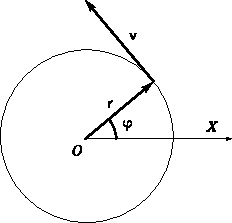
\includegraphics{figure/fig01.17}
    \caption{圆周运动}
    \label{fig:01.17}
\end{wrapfigure}
个意义上,两者是一样的。而一般的平面曲线运动,需要两个坐
标来描写;一般的空间曲线运动,则需要三个坐标来描写。我
们按描写运动所需坐标的个数,把运动分为一维运动、二维运动、
三维运动等等。直线运动和圆周运动都是一维运动。

按照\ref{sec:01.07}~节的讨论,速度的
方向为轨迹上相应点的切线方向,圆的切线总与半径相垂直,所
以圆周运动的速度$v$总与位置矢量$\vq{r}$相垂直。现在来求速度的

\begin{wrapfigure}[8]{l}{13em}
    \vspace{-0.5em}
    \centering \small
    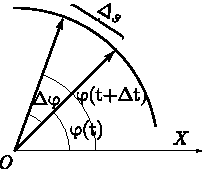
\includegraphics{figure/fig01.18}
    \caption{圆周运动的速率}
    \label{fig:01.18}
\end{wrapfigure}
\noindent 大小。由图\ref{fig:01.18},在$t$时刻,质点位于$\varphi(t)$;当$t+\Delta t$时,位于
$\varphi(t+\Delta t)$,所以在$\Delta t$间隔中质点
运动的路程为:
\setlength{\mathindent}{2em}
\begin{equation*}
    \begin{aligned}
        \Delta s &=r|\varphi(t+\Delta t)-\varphi(t)| \\
        &=r|\Delta \varphi|
    \end{aligned}
\end{equation*}
将此式代入式\eqref{eqn:01.07.05},就得到圆周运动的速率\vspace{-0.7em}
\setlength{\mathindent}{6em}
\begin{equation}\label{eqn:01.09.01}
    v=\lim _{\omega \rightarrow 0} \frac{r|\Delta \varphi|}{\Delta t}=r \lim _{\Delta \rightarrow 0} \frac{|\Delta \varphi|}{\Delta t}
\end{equation}
现在定义一个新的量,它是
\begin{equation}\label{eqn:01.09.02}
    \omega=\lim _{\Delta \rightarrow 0} \frac{|\Delta \varphi|}{\Delta t}
\end{equation}
这种形式的公式我们已经多次遇到了。$|\Delta\varphi|/\Delta t$是在$t$到$t+\Delta t$间
隔中,质点的单位时间的角位置的平均变化。当取$\Delta t\rightarrow 0$的极限
时,这个平均变化率过渡为瞬时变化率。因此,我们称$\omega$为角速
度,确切地说,应称为角速率。它的单位是弧度/秒。利用角速率$\varphi$,式\eqref{eqn:01.09.01}可以写成
\begin{equation}\label{eqn:01.09.03}
    v=r\omega
\end{equation}

速度本质上是一个矢量,有大小和方向两方面。上述角速度
定义只反映了大小,为反映方向,我们需作些补充。

现在定义一个矢量$\omega$,它的大小等于式\eqref{eqn:01.09.01}中的$\omega$,$\omega$的
方向按图\ref{fig:01.19}~所示的方法给定。
\begin{figure}[!h]
    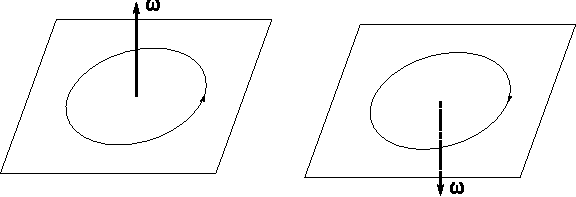
\includegraphics{figure/fig01.19}
    \caption{角速度的方向}
    \label{fig:01.19}
    \vspace{-1.2em}
\end{figure}

\noindent 当我们从$\omega$指向的方向观察质点的运动时,质点总是沿逆时钟方
向转动。这个规定$\omega$的方向的方法也可以用一个正扣螺旋来说
明,当螺钉按质点运动方向旋转时,螺钉的运动方向就是$\omega$的方
向。

这样定义的$\omega$,称为角速度矢量。利用这个矢量。可以把质
点的速度矢量$\vq{v}$表示成
\begin{equation}\label{eqn:01.09.04}
    \vq{v}=\omega\times \vq{r}
\end{equation}
由图\ref{fig:01.20},因为$\omega$与$\vq{r}$垂直,所以$|\omega\times\vq{r}|=\omega r=v$,
而且$|\omega\times\vq{r}|$的方向与$v$的方向一致。故式\eqref{eqn:01.09.04}
比\eqref{eqn:01.09.03}更具有一般性,它不仅表达了三者的大小关系,也反映了
三者间的方向关系。不仅如此,若取通过圆心且垂直于圆所在平面
的直线上任一点为原点(图\ref{fig:01.21})来描写圆周运动,式\eqref{eqn:01.09.04}仍成立,但式\eqref{eqn:01.09.03}就不对
\clearpage
\noindent 了。读者可以自己证明。

\begin{figure}[!h]
    \small
    \begin{minipage}[b]{15em}
        \centering
        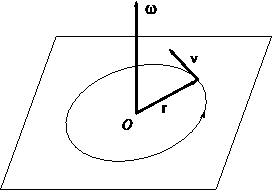
\includegraphics{figure/fig01.20}
        \vspace{4em}
        \caption{圆周运动中$\omega$与$v$的关系}
        \label{fig:01.20}
    \end{minipage}
    \hfill
    \begin{minipage}[b]{13em}
        \centering
        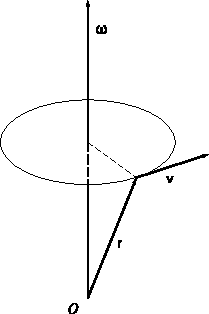
\includegraphics{figure/fig01.21}
        \vspace{1em}
        \caption{原点不在圆心的情况}
        \label{fig:01.21}
\end{minipage}
\end{figure}

